\documentclass{beamer}
\usepackage{amsmath,graphics}
\usepackage{amssymb}

\usetheme{default}
\usepackage{xcolor}

\definecolor{solarizedBase03}{HTML}{002B36}
\definecolor{solarizedBase02}{HTML}{073642}
\definecolor{solarizedBase01}{HTML}{586e75}
\definecolor{solarizedBase00}{HTML}{657b83}
\definecolor{solarizedBase0}{HTML}{839496}
\definecolor{solarizedBase1}{HTML}{93a1a1}
\definecolor{solarizedBase2}{HTML}{EEE8D5}
\definecolor{solarizedBase3}{HTML}{FDF6E3}
\definecolor{solarizedYellow}{HTML}{B58900}
\definecolor{solarizedOrange}{HTML}{CB4B16}
\definecolor{solarizedRed}{HTML}{DC322F}
\definecolor{solarizedMagenta}{HTML}{D33682}
\definecolor{solarizedViolet}{HTML}{6C71C4}
%\definecolor{solarizedBlue}{HTML}{268BD2}
\definecolor{solarizedBlue}{HTML}{134676}
\definecolor{solarizedCyan}{HTML}{2AA198}
\definecolor{solarizedGreen}{HTML}{859900}
\definecolor{myBlue}{HTML}{162DB0}%{261CA4}
\setbeamercolor*{item}{fg=myBlue}
\setbeamercolor{normal text}{fg=solarizedBase03, bg=solarizedBase3}
\setbeamercolor{alerted text}{fg=myBlue}
\setbeamercolor{example text}{fg=myBlue, bg=solarizedBase3}
\setbeamercolor*{frametitle}{fg=solarizedRed}
\setbeamercolor*{title}{fg=solarizedRed}
\setbeamercolor{block title}{fg=myBlue, bg=solarizedBase3}
\setbeameroption{hide notes}
\setbeamertemplate{note page}[plain]
\beamertemplatenavigationsymbolsempty
\usefonttheme{professionalfonts}
\usefonttheme{serif}

\usepackage{fourier}

\def\vec#1{\mathchoice{\mbox{\boldmath$\displaystyle#1$}}
{\mbox{\boldmath$\textstyle#1$}}
{\mbox{\boldmath$\scriptstyle#1$}}
{\mbox{\boldmath$\scriptscriptstyle#1$}}}

\definecolor{OwnGrey}{rgb}{0.560,0.000,0.000} % #999999
\definecolor{OwnBlue}{rgb}{0.121,0.398,0.711} % #1f64b0
\definecolor{red4}{rgb}{0.5,0,0}
\definecolor{blue4}{rgb}{0,0,0.5}
\definecolor{Blue}{rgb}{0,0,0.66}
\definecolor{LightBlue}{rgb}{0.9,0.9,1}
\definecolor{Green}{rgb}{0,0.5,0}
\definecolor{LightGreen}{rgb}{0.9,1,0.9}
\definecolor{Red}{rgb}{0.9,0,0}
\definecolor{LightRed}{rgb}{1,0.9,0.9}
\definecolor{White}{gray}{1}
\definecolor{Black}{gray}{0}
\definecolor{LightGray}{gray}{0.8}
\definecolor{Orange}{rgb}{0.1,0.2,1}
\setbeamerfont{sidebar right}{size=\scriptsize}
\setbeamercolor{sidebar right}{fg=Black}

\renewcommand{\emph}[1]{{\textcolor{solarizedRed}{\itshape #1}}}

\newcommand\cA{\mathcal A}
\newcommand\cB{\mathcal B}
\newcommand\cC{\mathcal C}
\newcommand\cD{\mathcal D}
\newcommand\cE{\mathcal E}
\newcommand\cF{\mathcal F}
\newcommand\cG{\mathcal G}
\newcommand\cH{\mathcal H}
\newcommand\cI{\mathcal I}
\newcommand\cJ{\mathcal J}
\newcommand\cK{\mathcal K}
\newcommand\cL{\mathcal L}
\newcommand\cM{\mathcal M}
\newcommand\cN{\mathcal N}
\newcommand\cO{\mathcal O}
\newcommand\cP{\mathcal P}
\newcommand\cQ{\mathcal Q}
\newcommand\cR{\mathcal R}
\newcommand\cS{\mathcal S}
\newcommand\cT{\mathcal T}
\newcommand\cU{\mathcal U}
\newcommand\cV{\mathcal V}
\newcommand\cW{\mathcal W}
\newcommand\cX{\mathcal X}
\newcommand\cY{\mathcal Y}
\newcommand\cZ{\mathcal Z}

\newcommand\fA{\mathfrak A}
\newcommand\fB{\mathfrak B}
\newcommand\fC{\mathfrak C}
\newcommand\fD{\mathfrak D}
\newcommand\fE{\mathfrak E}
\newcommand\fF{\mathfrak F}
\newcommand\fG{\mathfrak G}
\newcommand\fH{\mathfrak H}
\newcommand\fI{\mathfrak I}
\newcommand\fJ{\mathfrak J}
\newcommand\fK{\mathfrak K}
\newcommand\fL{\mathfrak L}
\newcommand\fM{\mathfrak M}
\newcommand\fN{\mathfrak N}
\newcommand\fO{\mathfrak O}
\newcommand\fP{\mathfrak P}
\newcommand\fQ{\mathfrak Q}
\newcommand\fR{\mathfrak R}
\newcommand\fS{\mathfrak S}
\newcommand\fT{\mathfrak T}
\newcommand\fU{\mathfrak U}
\newcommand\fV{\mathfrak V}
\newcommand\fW{\mathfrak W}
\newcommand\fX{\mathfrak X}
\newcommand\fY{\mathfrak Y}
\newcommand\fZ{\mathfrak Z}

\newcommand\fa{\mathfrak a}
\newcommand\fb{\mathfrak b}
\newcommand\fc{\mathfrak c}
\newcommand\fd{\mathfrak d}
\newcommand\fe{\mathfrak e}
\newcommand\ff{\mathfrak f}
\newcommand\fg{\mathfrak g}
\newcommand\fh{\mathfrak h}
%\newcommand\fi{\mathfrak i}
\newcommand\fj{\mathfrak j}
\newcommand\fk{\mathfrak k}
\newcommand\fl{\mathfrak l}
\newcommand\fm{\mathfrak m}
\newcommand\fn{\mathfrak n}
\newcommand\fo{\mathfrak o}
\newcommand\fp{\mathfrak p}
\newcommand\fq{\mathfrak q}
\newcommand\fr{\mathfrak r}
\newcommand\fs{\mathfrak s}
\newcommand\ft{\mathfrak t}
\newcommand\fu{\mathfrak u}
\newcommand\fv{\mathfrak v}
\newcommand\fw{\mathfrak w}
\newcommand\fx{\mathfrak x}
\newcommand\fy{\mathfrak y}
\newcommand\fz{\mathfrak z}

\newcommand\vA{\vec A}
\newcommand\vB{\vec B}
\newcommand\vC{\vec C}
\newcommand\vD{\vec D}
\newcommand\vE{\vec E}
\newcommand\vF{\vec F}
\newcommand\vG{\vec G}
\newcommand\vH{\vec H}
\newcommand\vI{\vec I}
\newcommand\vJ{\vec J}
\newcommand\vK{\vec K}
\newcommand\vL{\vec L}
\newcommand\vM{\vec M}
\newcommand\vN{\vec N}
\newcommand\vO{\vec O}
\newcommand\vP{\vec P}
\newcommand\vQ{\vec Q}
\newcommand\vR{\vec R}
\newcommand\vS{\vec S}
\newcommand\vT{\vec T}
\newcommand\vU{\vec U}
\newcommand\vV{\vec V}
\newcommand\vW{\vec W}
\newcommand\vX{\vec X}
\newcommand\vY{\vec Y}
\newcommand\vZ{\vec Z}

\newcommand\va{\vec a}
\newcommand\vb{\vec b}
\newcommand\vc{\vec c}
\newcommand\vd{\vec d}
\newcommand\ve{\vec e}
\newcommand\vf{\vec f}
\newcommand\vg{\vec g}
\newcommand\vh{\vec h}
\newcommand\vi{\vec i}
\newcommand\vj{\vec j}
\newcommand\vk{\vec k}
\newcommand\vl{\vec l}
\newcommand\vm{\vec m}
\newcommand\vn{\vec n}
\newcommand\vo{\vec o}
\newcommand\vp{\vec p}
\newcommand\vq{\vec q}
\newcommand\vr{\vec r}
\newcommand\vs{\vec s}
\newcommand\vt{\vec t}
\newcommand\vu{\vec u}
\newcommand\vv{\vec v}
\newcommand\vw{\vec w}
\newcommand\vx{\vec x}
\newcommand\vy{\vec y}
\newcommand\vz{\vec z}

\newcommand\NN{\mathbb N}
\newcommand\ZZ{\mathbb Z}
\newcommand\PP{\mathbb P}
\newcommand\QQ{\mathbb Q}
\newcommand\RR{\mathbb R}
\newcommand\CC{\mathbb C}

\newcommand{\pr}{\mathrm{P}}
\newcommand{\Vol}{\mathrm{vol}}
\newcommand\norm[1]{\left\|{#1}\right\|} 
\newcommand\sign{\mathrm{sign}}
\newcommand{\eps}{\varepsilon}
\newcommand{\abs}[1]{\left|#1\right|}
\newcommand\bc[1]{\left({#1}\right)} 
\newcommand\cbc[1]{\left\{{#1}\right\}} 
\newcommand\bcfr[2]{\bc{\frac{#1}{#2}}} 
\newcommand{\bck}[1]{\left\langle{#1}\right\rangle} 
\newcommand\brk[1]{\left\lbrack{#1}\right\rbrack} 
\newcommand\scal[2]{\bck{{#1},{#2}}} 
\newcommand{\vecone}{\mathbb{1}}
\newcommand{\tensor}{\otimes}
\newcommand{\diag}{\mathrm{diag}}
\newcommand{\ggt}{\mathrm{ggT}}
\newcommand{\kgv}{\mathrm{kgV}}

\newcommand{\Karonski}{Karo\'nski}
\newcommand{\Erdos}{Erd\H{o}s}
\newcommand{\Renyi}{R\'enyi}
\newcommand{\Lovasz}{Lov\'asz}
\newcommand{\Juhasz}{Juh\'asz}
\newcommand{\Bollobas}{Bollob\'as}
\newcommand{\Furedi}{F\"uredi}
\newcommand{\Komlos}{Koml\'os}
\newcommand{\Luczak}{\L uczak}
\newcommand{\Kucera}{Ku\v{c}era}
\newcommand{\Szemeredi}{Szemer\'edi}

\renewcommand{\ae}{\"a}
\renewcommand{\oe}{\"o}
\newcommand{\ue}{\"u}
\newcommand{\Ae}{\"A}
\newcommand{\Oe}{\"O}
\newcommand{\Ue}{\"U}

\title[Linadi]{Der Primzahlsatz}
\author[Amin Coja-Oghlan]{Amin Coja-Oghlan}
\institute[Frankfurt]{JWGUFFM}
\date{}

\begin{document}

\frame[plain]{\titlepage}

\begin{frame}\frametitle{Der Primzahlsatz}
	\hfill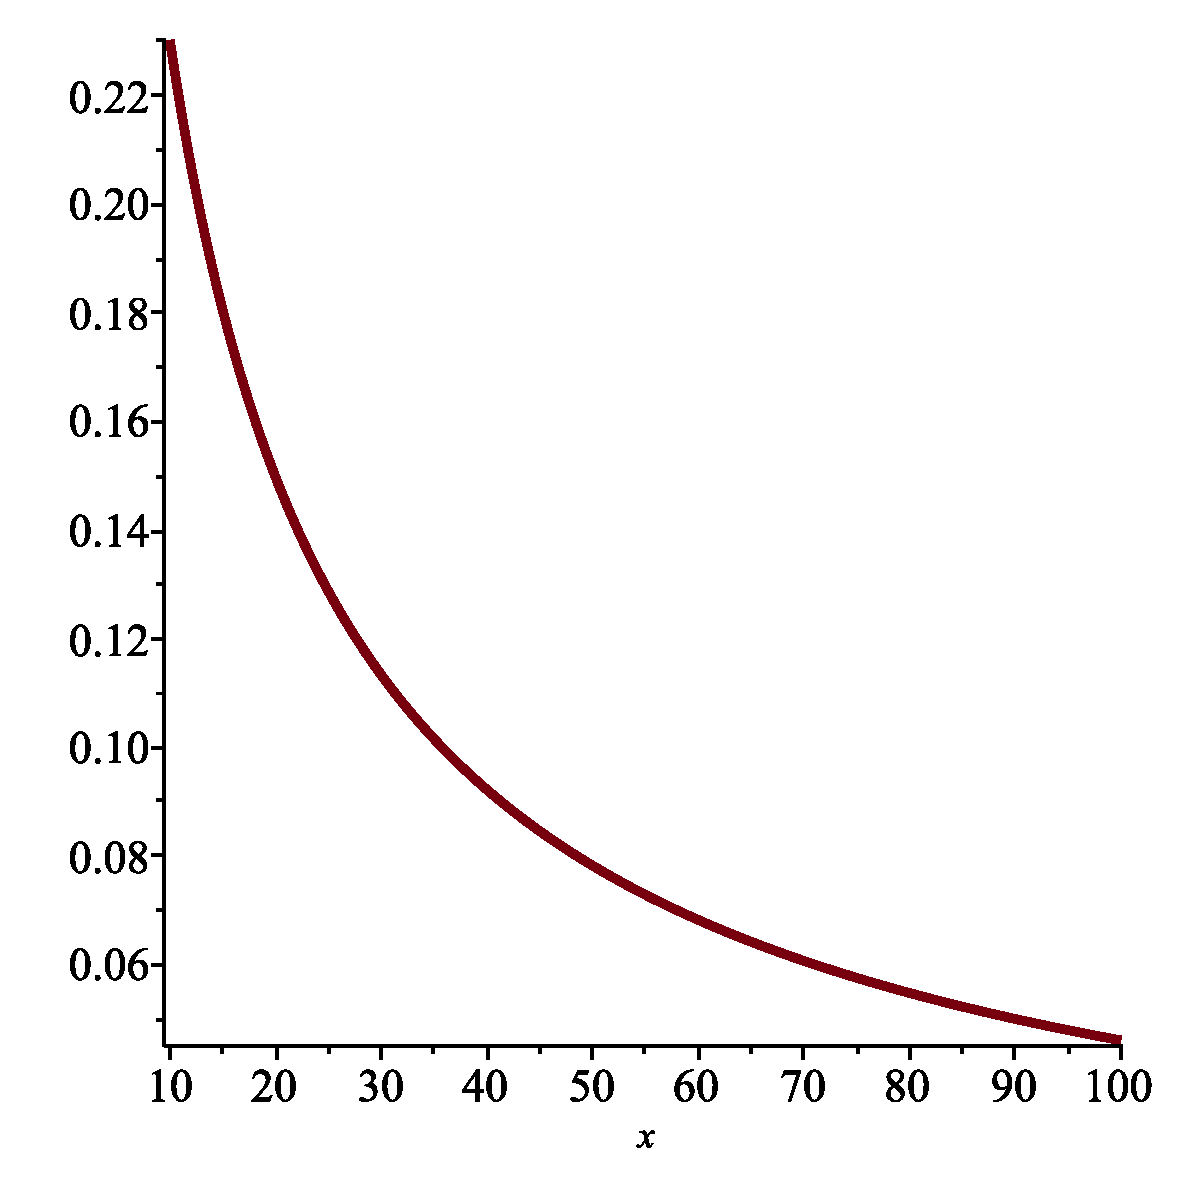
\includegraphics[height=30mm]{pics/pnt.eps}
	\begin{block}{Satz}
		Es gibt eine Zahl $N\in\NN$, so da\ss\ f\ue r alle $n>N$ gilt:
		\begin{align*}
		\abs{\cbc{p\in\PP:n\leq p<2n}}\geq\frac{n}{N\log n}.
		\end{align*}
	\end{block}

	\bigskip
	{\itshape Erinnerung: $\log(x)$ bezeichnet den nat\ue rlichen Logarithmus von $x>0$, definiert als $\log(x)=\int_0^x\frac{\mathrm dt}{t}$.}
\end{frame}

\begin{frame}\frametitle{Der Primzahlsatz}
	\hfill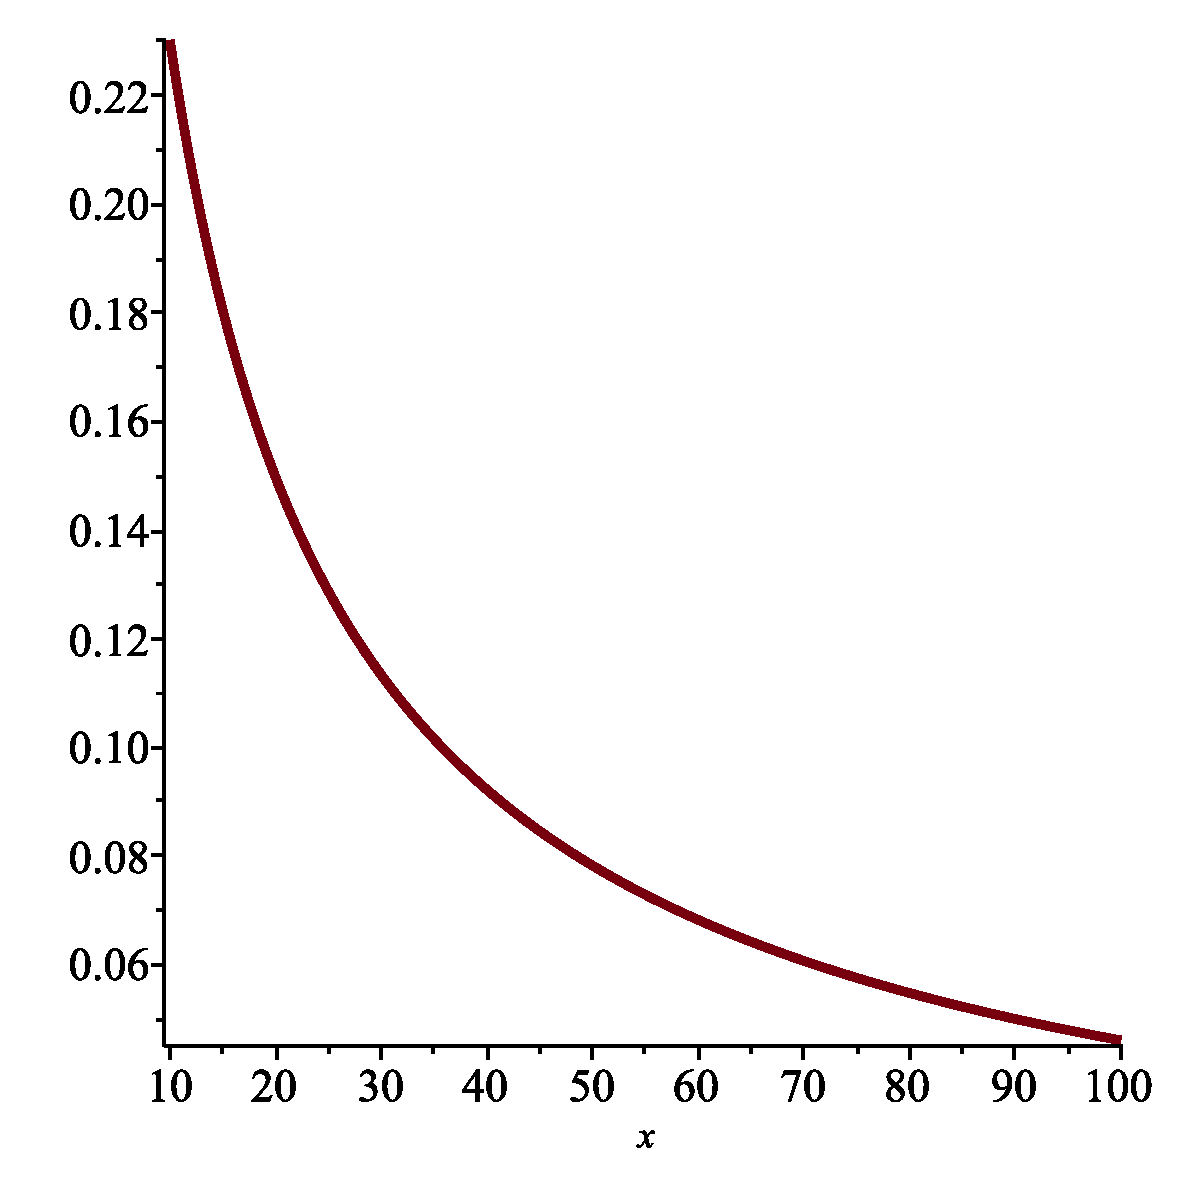
\includegraphics[height=30mm]{pics/pnt.eps}
	\begin{block}{Satz}
		Es gibt eine Zahl $N\in\NN$, so da\ss\ f\ue r alle $n>N$ gilt:
		\begin{align*}
		\abs{\cbc{p\in\PP:n\leq p<2n}}\geq\frac{n}{N\log n}.
		\end{align*}
	\end{block}

	\bigskip
	\emph{Anmerkung:} der `erwachsene' Primzahlsatz besagt, da\ss\
	\begin{align*}
		\lim_{n\to\infty}\abs{\cbc{p\in\PP:p\leq n}}\cdot\frac{\log n}{n}&=1.
	\end{align*}
\end{frame}

\begin{frame}\frametitle{Lemma~1}
\begin{block}{Lemma}
	F\ue r alle $n\in\NN$ gilt $\prod_{p\in\PP:1<p\leq n}p\leq 4^{n-1}$.
\end{block}
\begin{block}{Beweis}
\begin{itemize}
\item Induktion nach $n$; die F\ae lle $n=1,2$ sind klar.
\item Wir nehmen an, da\ss\ $n=2q+1$ selbst prim ist.
\item Wir zerlegen das Produkt in  	$\prod_{p\in\PP:1<p\leq n}p=P_1\cdot P_2$ mit
	\begin{align*}
		P_1=&\prod_{p\in\PP:1<p\leq q+1}p,\quad P_2=\prod_{p\in\PP:q+1<p\leq n}p.
	\end{align*}
\item Nach Induktion gilt $P_1\leq 4^q$.
\end{itemize}
\end{block}
\end{frame}

\begin{frame}\frametitle{Lemma~1}
\begin{block}{Beweis (Fortsetzung)}
\begin{itemize}
\item F\ue r jede Primzahl $p>q+1$ gilt ferner
	\begin{align*}
		w_p\binom nq\geq w_p(n);
	\end{align*}
	denn $\binom nq=\frac{n!}{q!(q+1)!}\in\NN$ und $p\nmid(q+1)!$.
\item Also schlie\ss en wir, da\ss\
	\begin{align*}
		P_2\leq\binom nq\leq 2^{n-1};
	\end{align*}
	die letzte Ungleichung gilt, weil $\binom nq=\binom n{q+1}$ und $\binom nq+\binom n{q+1}\leq 2^n$ nach dem binomischen Lehrsatz.
\item Wir erhalten die Behauptung, indem wir die Schranken f\ue r $P_1,P_2$ kombinieren.
\end{itemize}
\end{block}
\end{frame}

\begin{frame}\frametitle{Lemma~2}
\begin{block}{Lemma}
	F\ue r jede Primzahl $p>1$ gilt $w_p(n!)=\sum_{k\geq1}\lfloor n/p^k\rfloor$.
\end{block}
\begin{block}{Beweis}
\begin{itemize}
	\item Unter den Zahlen $1,\ldots,n$ sind genau $\lfloor n/p^k\rfloor$ durch $p^k$ teilbar.
	\item Aufsummieren \ue ber $k$ liefert die Behauptung.
\end{itemize}
\end{block}
\end{frame}

\begin{frame}\frametitle{Lemma~3}
	\begin{block}{Lemma}
		F\ue r alle $n\in\NN$ und alle Primzahlen $p>1$ gilt 
		\begin{align*}
			w_p\binom{2n}n\leq\max\cbc{r\geq0:p^r\leq2n}.
		\end{align*}
		Au\ss erdem gilt $p\nmid\binom{2n}n$, falls $2n/3<p\leq n$.
	\end{block}
	\begin{block}{Beweis}
		\begin{itemize}
			\item Aus Lemma~2 schlie\ss en wir, da\ss 
				\begin{align*}
					w_p\binom{2n}n=w_p((2n)!)-2w_p(n!)=\sum_{k\geq1}\lfloor 2n/p^k\rfloor-2\lfloor n/p^k\rfloor.
				\end{align*}
			\item Weil $\lfloor 2n/p^k\rfloor-2\lfloor n/p^k\rfloor\leq1$ und $\lfloor 2n/p^k\rfloor=\lfloor n/p^k\rfloor=0$ f\ue r $p^k>2n$, erhalten wir die erste Behauptung.
		\end{itemize}
	\end{block}
\end{frame}

\begin{frame}\frametitle{Lemma~3}
	\begin{block}{Beweis (Fortsetzung)}
		\begin{itemize}
			\item Nimm nun an, da\ss\ $2n/3<p\leq n$.
			\item Dann enth\ae lt $(2n)!$ nur die Vielfachen $p,2p$.
			\item Ferner enth\ae lt $n!$ einen Faktor $p$.
			\item Folglich k\ue rzt sich $p$ aus
				\begin{align*}
					\binom{2n}n=\frac{(2n)!}{n!^2}
				\end{align*}
				komplett heraus.
		\end{itemize}
	\end{block}
\end{frame}

\begin{frame}\frametitle{Beweis des Satzes}
	\begin{itemize}
		\item Aus Lemma~3 folgt, da\ss\ 
			\begin{align*}
				\binom{2n}n&=\prod_{p\in\PP:1<p<2n}p^{w_p\binom{2n}n}\leq Q_1Q_2Q_3\qquad\mbox{mit}\\
				Q_1&=\prod_{p\leq\sqrt{2n}}(2n),\ Q_2=\prod_{\sqrt{2n}<p<2n/3}p,\ Q_3=\prod_{n<p\leq 2n}p.
			\end{align*}
		\item F\ue r hinreichend gro\ss e $n$ gilt 
			\begin{align*}
				Q_1\leq (2n)^{\sqrt{2n}}=\exp(\sqrt{2n}\log(2n))\leq 4^{n/6}.
			\end{align*}
		\item Au\ss erdem zeigt Lemma~1, da\ss\ 
			\begin{align*}
				Q_2\leq \prod_{1<p\leq 2n/3}p\leq 4^{2n/3}.
			\end{align*}
		\item Also schlie\ss en wir, da\ss\ 
			\begin{align*}
				Q_3\geq 4^{-2n/3-n/6}\binom{2n}n=4^{-5n/6}\binom{2n}n.
			\end{align*}
	\end{itemize}
\end{frame}

\begin{frame}\frametitle{Beweis des Satzes}
	\begin{itemize}
		\item Aus dem binomischen Lehrsatz folgt f\ue r gro\ss e $n$
			\begin{align*}
				\binom{2n}n\geq 4^n/n\geq 4^{11n/12}.
			\end{align*}
		\item Also erhalten wir
			\begin{align*}
				\prod_{n<p\leq 2n}p=Q_3\geq 4^{n/12}.
			\end{align*}
		\item Weil jeder der Faktoren durch $2n$ beschr\ae nkt ist, mu\ss\ f\ue r die Anzahl der Faktoren gelten, da\ss\
			\begin{align*}
				\abs{\cbc{p\in\PP:n<p\leq 2n}}\geq\frac{n}{12\log(n)}.
			\end{align*}
	\end{itemize}
\end{frame}

\begin{frame}\frametitle{Zusammenfassung}
\begin{itemize}
\item Der Primzahlsatz bestimmt die ungef\ae hre Anzahl der Primzahlsatz bis zu einer bestimmten Zahl $n$.
\item Wenn wir eine Zahl aus $\{1,\ldots,n\}$ zuf\ae llig ausw\ae hlen, ist die Wahrscheinlichkeit, eine Primzahl zu treffen, etwa $1/\log n$.
\end{itemize}
\end{frame}

\end{document}
